\documentclass[10pt]{article}


\usepackage[utf8]{inputenc}
\usepackage[T1]{fontenc}
\usepackage[frenchb]{babel}

\usepackage{algorithm}
\usepackage{algorithmic}
\usepackage[T1]{fontenc}
\usepackage{enumitem}
\usepackage{hyperref}
\usepackage{graphicx}
\usepackage{color}
\usepackage{listings}
\usepackage{wrapfig}
\usepackage{amsfonts}
\usepackage{amsmath}
\usepackage{mathtools}
\usepackage[hmargin=1.25in,vmargin=1.25in]{geometry}
\usepackage{framed}
\usepackage{mathenv}
\usepackage{blkarray}

%title setuplisting
\title{Projet WEB de groupe}
\author{
  Gangyue CHEN \\
  Louis LAFUMA \\
  Baptiste LAMBERT \\
  Romain PEREIRA
}
\date{22/05/2018}

% table of contents setup
\renewcommand{\contentsname}{Sommaire}
\usepackage{etoolbox}
\patchcmd{\thebibliography}{\section*{\refname}}{}{}{}

\setlength{\parindent}{0cm}
\setlength{\parskip}{1ex plus 0.5ex minus 0.2ex}
\newcommand{\hsp}{\hspace{20pt}}
\newcommand{\HRule}{\rule{\linewidth}{0.5mm}}

\hypersetup{
  colorlinks,
  citecolor=black,
  filecolor=black,
  linkcolor=blue,
  urlcolor=red
}

\begin{document}
  \begin{titlepage}
    \begin{sffamily}
      \begin{center}
	
	\textsc{\LARGE ENSIIE}\\[2cm]
	\textsc{\Large Rapport de projet}\\[1.5cm]
	% Title
	\HRule \\[0.4cm]
	{ \huge \bfseries Projet web en groupe ENSIIE 1A 2018\\[0.4cm] }
	\HRule \\[2cm]
	
	\begin{minipage}{0.4\textwidth}
	  \begin{flushleft} \large
	    Guangyue \textsc{Chen}\\
	    Louis \textsc{Lafuma}\\
	    Baptiste \textsc{Lambert}\\
	    Romain \textsc{Pereira}\\
	  \end{flushleft}
	\end{minipage}
	\begin{minipage}{0.4\textwidth}
	  \begin{flushright} \large
	    \emph{Encadrants :} \\
	    Thomas \textsc{Comes}\\
	    Nassim \textsc{Kirouane}\\
	    Rémi \textsc{Parpaillon}\\
	  \end{flushright}
	\end{minipage}
	\vfill
	% Bottom of the page
	{\large 22/05/2018}
      \end{center}
    \end{sffamily}
  \end{titlepage}
  \maketitle
  \tableofcontents
  
  \section*{Préambule}
  Ce projet est réalisé dans le cadre de nos études à l'ENSIIE.
  Les objectifs sont d'apprendre à concevoir et développer des applications web utilisant un serveur de bases de données,
  et prendre conscience des problématiques d’organisations d’équipes et de répartition des tâches.
  
  \newpage
  \section{La problématique}
  
  \newpage
  \section{Solution technique}
    \subsection{Répartition des rôles}
    \subsection{Back-end}
      La base de données est relationelle (language SQL).
      \newline
      Elle peut être representé par le diagramme UML suivant:
      \begin{figure}[H]
	\begin{center}
	  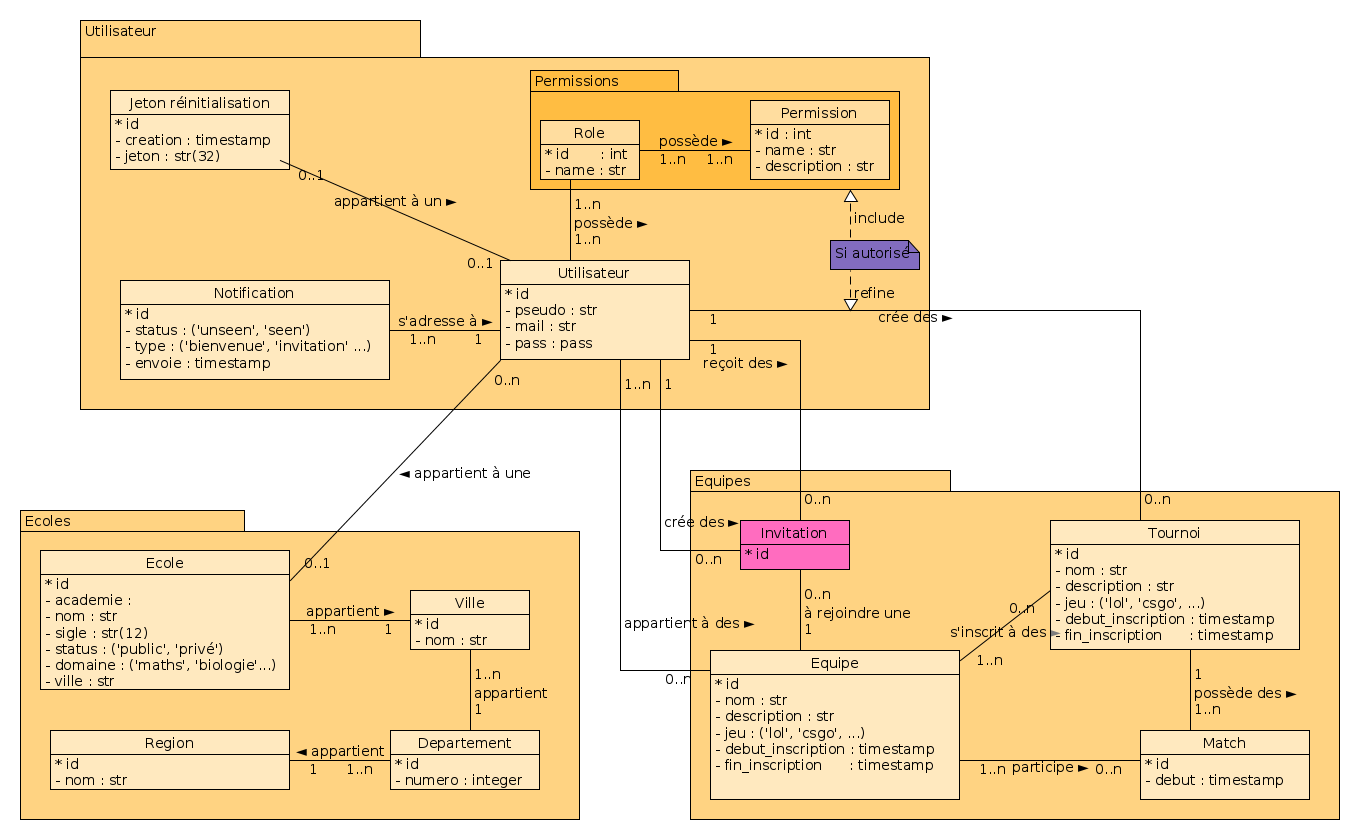
\includegraphics[width=18cm,keepaspectratio]{./images/uml.png}
	\end{center}
	\caption{\textit{Schéma UML de la base de données}}
	\label{uml}
      \end{figure}
      
      La transcription SQL du modèle est disponible dans le fichier 'data/db.sql'.
      
      \subsubsection{Utilisateur}
	\paragraph{Permission}
	\paragraph{Utilisateur}
	\paragraph{Notification}
	\paragraph{Jeton de réinitialisation}
      
      \subsubsection{Ecoles}
	Une base de données a été généré à partir de la page Wikipédia \ref{ecole_ingé}.
	Les données ont été extraite de la page, au format csv, à l'aide d'un programme Python (et de la bibliothèque BeautifulSoup \ref{beautifulsoup}).
	
	Cette base de donnée aura 2 utilités principales : auto-complétion pour la recherche, et organisation de tournois par région.
	Elle permettra également d'avoir des statistiques par région (fait t'on plus d'e-sport à Angers ou bien à Paris?).
	
      \subsubsection{Equipes}
	\paragraph{Equipe}
	\paragraph{Tournoi}
	\paragraph{Match}
	\paragraph{Invitation}

    \subsection{Front-end}
  \newpage
  \section{Conclusion}
  
  \newpage
  \section{Références}
  \begin{thebibliography}{}
    
    \bibitem{phpgoodpratices}\label{phpgoodpratices}
    'PHP The Right Way' - \href{https://github.com/codeguy/php-the-right-way/graphs/contributors}{\textit{+200 authors}} \newline
    \href{http://www.phptherightway.com/}{\textit{http://www.phptherightway.com/}}
    
    \bibitem{riotapi}\label{riotapi}
    API officiel de Riot Games\newline
    \href{https://developer.riotgames.com/}{\textit{https://developer.riotgames.com/}}
    
    \bibitem{discordapi}\label{discordapi}
    API officiel de Discord\newline
    \href{https://discordapp.com/developers/docs/intro}{\textit{https://discordapp.com/developers/docs/intro}}
    
    \bibitem{ecole_ingé}\label{ecole_ingé}
    Liste écoles d'ingénieur en France - Wikipédia\newline
    \href{https://fr.wikipedia.org/wiki/Liste_des_écoles_d'ingénieurs_en_France#Liste_des_207_écoles_françaises_accréditées_au_1er_septembre_2017}{\textit{https://fr.wikipedia.org/wiki/Liste\_des\_écoles\_d'ingénieurs\_en\_France}}
    
    \bibitem{beautifulsoup}\label{beautifulsoup}
    BeautifulSoup - Documentation\newline
    \href{https://www.crummy.com/software/BeautifulSoup/bs4/doc/}{\textit{https://www.crummy.com/software/BeautifulSoup/bs4/doc/}}
    
  \end{thebibliography}
  
\end{document}
